\section{System Dynamics Model} \label{section:model}
This chapter provide explanation and details regarding the developed model in Vensim. Before further scrutinize the implementation and for the sake of simplicity \textbf{some of the variable definitions are going to be presented as graphs}. This is because, as stated before, \textbf{this study is mostly based on the results of surveys}, hence, the best way to define some of the variables is to use the resulting data form those surveys, instead of a pure mathematical definition.

In the \textbf{cases where the variables function were define through data}, this \textbf{data was based from \cite{thesis-base, pedro-report} and adapted to the Portuguese scenario and reality using external sources}, such as news articles \cite{dv-news-article, eco-news-article, obs-news-article, uve-news-article}. Finally, to implement this types of variable functions, it was used the feature \textbf{Lookups} of Vensim, showcased in section \cite{vensim-youtube-lookups}.

\subsection{Proposed System Dynamics Model}
An can be seen in the figure \ref{fig:vensim-model}, the developed model takes into account all the factors discussed in section \ref{section:factors}.

\begin{figure}[!htbp]
\centerline{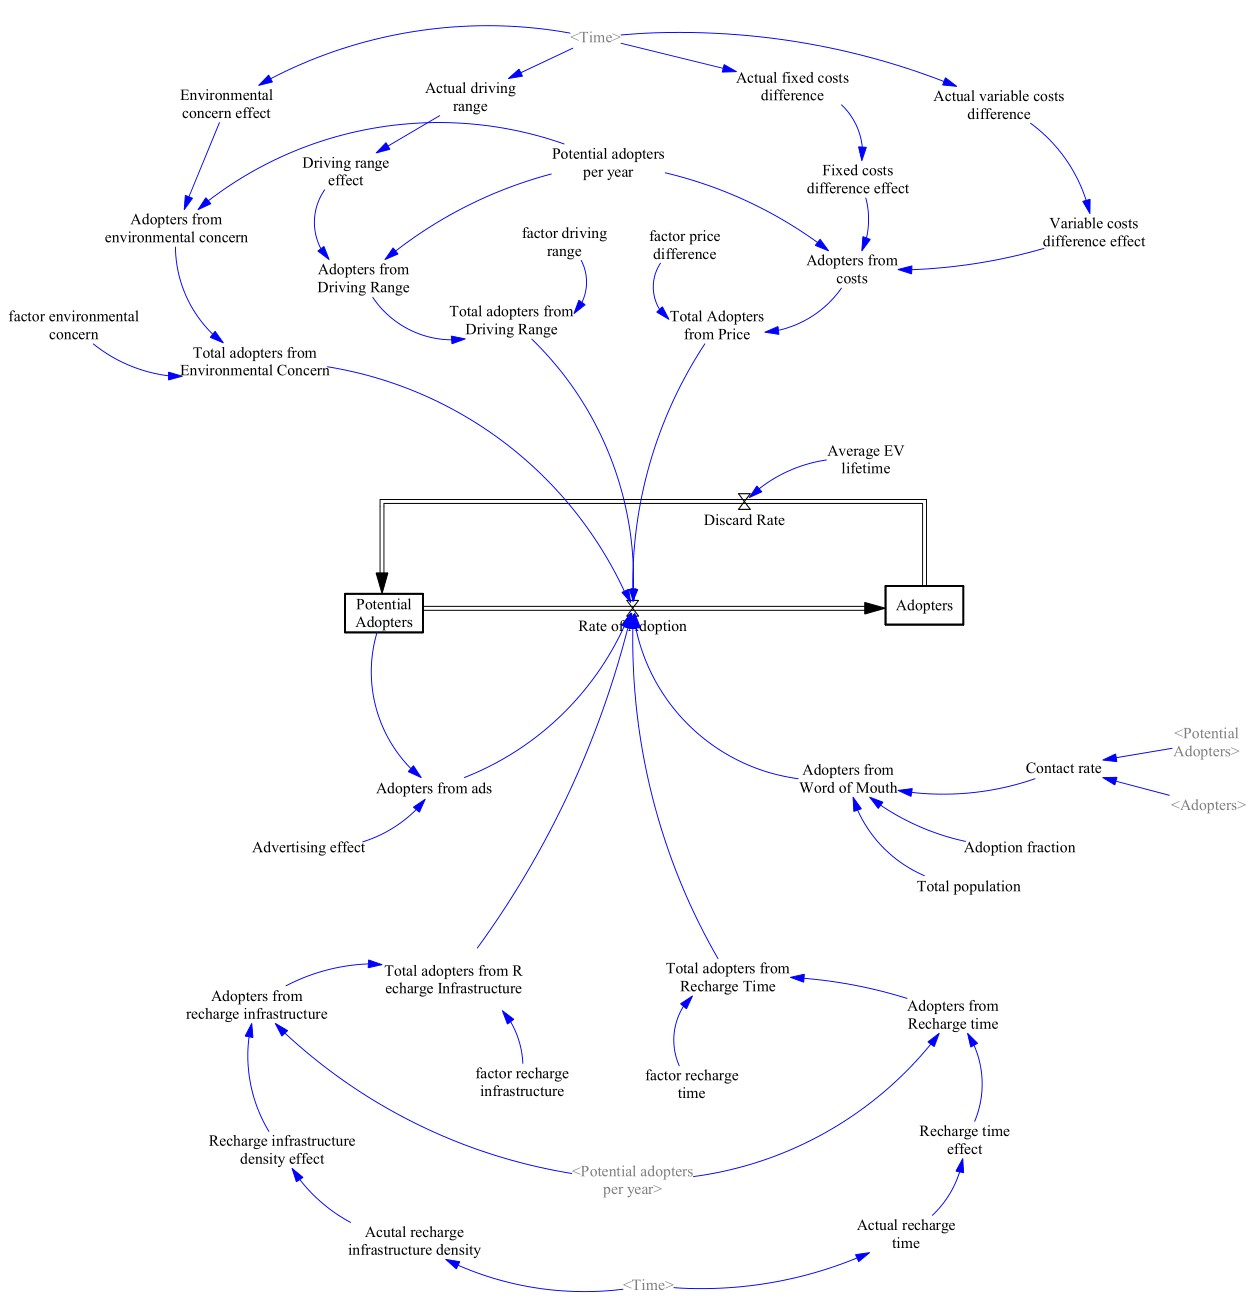
\includegraphics[width=0.74\linewidth]{img/vensim-model.jpg}}
\caption{Complete Model of EV Adoption Process}
\label{fig:vensim-model}
\end{figure}

\clearpage

Before going into detail on each factor representation and associated relationships, let's first explore the adopted layout with \textbf{Potential Adopters $\rightarrow$ Actual Adopters} and \textbf{Discard Rate}.

\subsubsection{Potential Adopters $\rightarrow$ Actual Adopters}
This model starts with the potential adopters, which are the current passenger vehicle drivers and account for approximately 6.5 million Portuguese drivers. Taking the model into consideration we can clearly see that through the rate of adoption, a fraction of these 6.5 million drivers will become adopters each ear, that is, will purchase an EV. The adopters variable has an initial value of 16 000 drivers, that represents the Portuguese drivers that already have an electric vehicle in 2020. 

\subsubsection{Discard Rate}
The bass diffusion model is frequently described as a \textit{first-purchase} model because it does not grasp the situation where the product is consumed, upgraded or discarded. What this means is that the bass diffusion model is not able to represent the inverse situation (Actual Adopters $\rightarrow$ Potential Adopters). The implemented model has the capability to capture that situation in the sense that an EV can, for instance be discarded or upgraded due to the battery lifetime or dissatisfaction. This event is modelled with the battery lifetime that has a value of 15 years. 

\subsection{Variables Definition}
The \textbf{variables} that are going to be \textbf{explored with more detail in the next sub-chapters are} the ones that were \textbf{based on data from the surveys}. It is going to be presented the graphs associated with each one of these variables and will also be explored its context beyond the number representation. All the remaining variables (that are simple mathematical functions or constants) are summarized in the table \ref{table:model-summary}, further ahead.

\subsubsection{Driving Range}
Given the current average capacity of the batteries on the market and the past years of evolution, figure \ref{fig:driving-range} describes the current average of EV's maximum range at 250km, at year 0 (2020), and an evolution to 300km after 5 years (2025), all the way to 675km at 2040. Obviously the further we predict, the less reliable are those predictions, so some of these number are, as said, just predictions and can be wrong, but are the best possible predictions given the data we have today.

Figure \ref{fig:driving-range-effect} shows us the acceptance percentages of EVs maximum range according to the consumer's responses on the surveys. The graph shows us that, even today, the average driving range it's not very well accepted, since only 5\% - 10\% of the enquired customers would buy a vehicle with that range. The minimum driving range that has a certain degree of acceptance is 440km, so it can be expected that this factor could have a big positive impact on EV sales from 2030. Obviously this is not the only factor to consider as we will see further ahead that a good recharge infrastructure with high charging speeds could lessen the need for higher driving range values.

\vspace{2cm}

\begin{figure}[htbp]
\centering
\begin{subfigure}{0.5\textwidth}
  \centering
  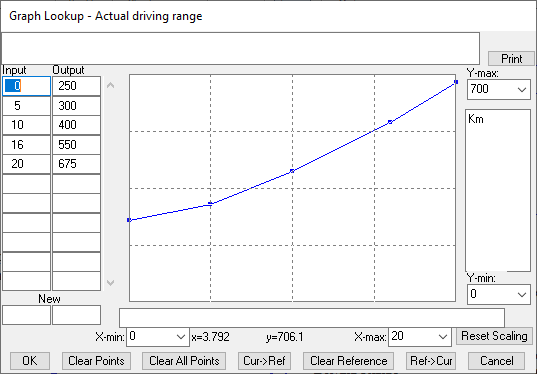
\includegraphics[width=0.98\linewidth]{img/driving-range.png}
  \caption{Actual Driving Range Data}
  \label{fig:driving-range}
\end{subfigure}%
\begin{subfigure}{0.5\textwidth}
  \centering
  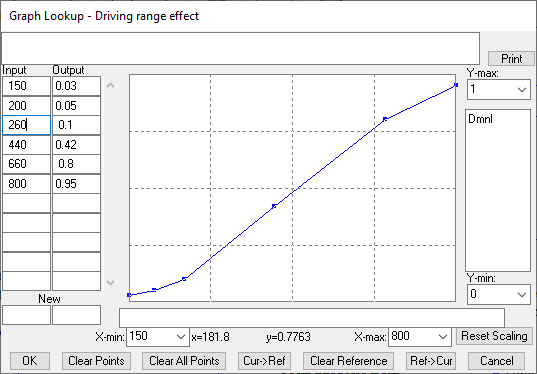
\includegraphics[width=0.98\linewidth]{img/driving-range-effect.png}
  \caption{Driving Range Effect Data}
  \label{fig:driving-range-effect}
\end{subfigure}
\caption{Driving Range Functions}
\label{fig:driving-range-funcs}
\end{figure}

\subsubsection{Price}
Considering the high costs of the lithium-ion batteries, electric vehicles tend to have a higher selling price than combustion models of the same range. Figure \ref{fig:fixed-costs} shows us precisely that. At 2020, 0-year, the average price difference between an EV and an ICV is 10 000\euro, which means that, an electric vehicle costs 10 000\euro \space more than a similar ICV model. After 5 years, this difference is around 5000\euro, that is, in 5 years the difference of prices has reduced over 50\%. At 2040 the price difference is in all-time low of 1900\euro, reducing the price difference to 20\% of its initial value.

\begin{figure}[htbp]
\centering
\begin{subfigure}{0.5\textwidth}
  \centering
  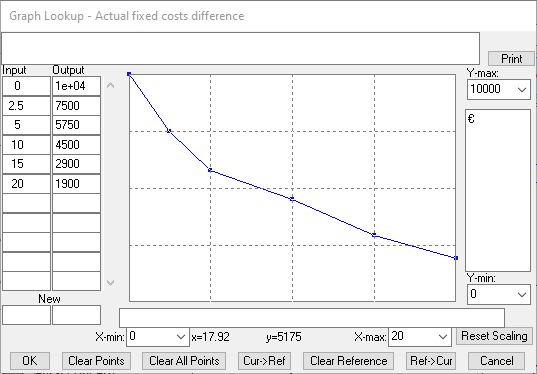
\includegraphics[width=0.98\linewidth]{img/fixed-costs-difference.png}
  \caption{Actual Fixed Costs Difference Data}
  \label{fig:fixed-costs}
\end{subfigure}%
\begin{subfigure}{0.5\textwidth}
  \centering
  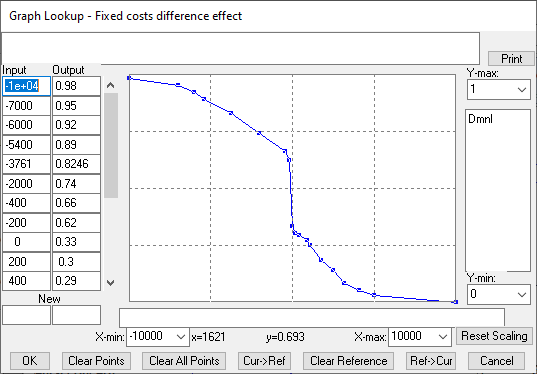
\includegraphics[width=0.98\linewidth]{img/fixed-costs-difference-effect.png}
  \caption{Fixed Costs Difference Effect Data}
  \label{fig:fixed-costs-effect}
\end{subfigure}
\caption{Fixed Costs Difference Functions}
\label{fig:fixed-costs-funcs}
\end{figure}

Figure \ref{fig:fixed-costs-effect} shows us the acceptance percentages of these differences in price regarding EV and ICV models. From the graph, we can understand that the majority of people can only consider purchase an EV when its price is the same or less than an equivalent ICV. If we would only consider this factor, we would wrongly think that, even 20 years from now, only a minority of the population would buy an EV. The aspect that we must have in consideration is the variable costs such as oil pricing, government subsidies and/or tax the reduction, electricity price. Some of these factors significantly amortize the price difference, either instantly or over time.

\subsubsection{Recharge Infrastructure}
As said before, the recharge infrastructure is the network of recharging stations (public or private, that is, home recharge "stations" are considered as private stations) scattered all over the country and it is one of the most important differences between the EV and ICV markets. As figure \ref{fig:recharge-infra} clearly demonstrates, today we have an average density of 100km between each station and this value is actually deceitful, because it does not represent evenly all Portuguese territory. The predictions suggest that in 20 years, Portugal will have an average density of recharge stations around 0km - 5km, which is actually very optimistic.

\begin{figure}[htbp]
\centering
\begin{subfigure}{0.5\textwidth}
  \centering
  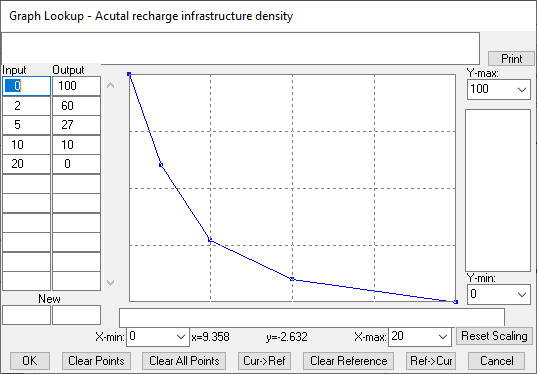
\includegraphics[width=0.98\linewidth]{img/recharge-infra-density.png}
  \caption{Actual Recharge Infrastructure Density Data}
  \label{fig:recharge-infra}
\end{subfigure}%
\begin{subfigure}{0.5\textwidth}
  \centering
  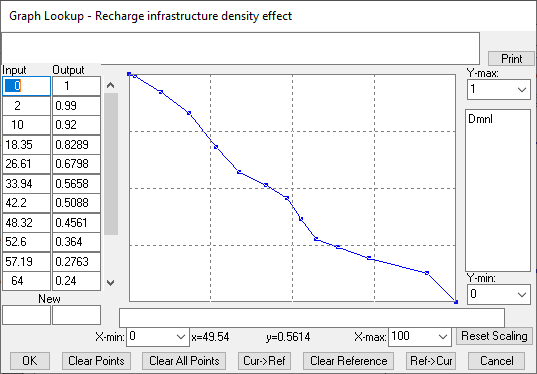
\includegraphics[width=0.98\linewidth]{img/recharge-infra-density-effect.png}
  \caption{Recharge Infrastructure Density Effect Data}
  \label{fig:recharge-infra-effect}
\end{subfigure}
\caption{Recharge Infrastructure Density Functions}
\label{fig:recharge-infra-funcs}
\end{figure}

Figure \ref{fig:recharge-infra-effect} allows us to better understand what the consumer thinks of this factor. According the surveys, the great majority of the population believes that the acceptable recharge infrastructure density is between 0km and 40km.

\subsubsection{Recharging Time}
If we own an ICV and we are close to run out of fuel, the process of refuel our vehicle could not be simpler or faster, taking no more than 5 minutes to fill the tank. In the case of electric vehicles the currently reality is not quite the same, since, currently, the action of completely recharging a EV can take up to 6,5 hours. Figure \ref{fig:recharge-time}, show us that 5 years from now, the process of recharge an EV could be less time consuming, taking at most 5 hours to fully charge an EV and that 20 years from now the same process will be significantly faster taking 2 minutes to be completed, thanks to the switch of a discharged battery (that will be promptly recharged) for a fully charged one.

In figure \ref{fig:recharge-time-effect} we can see that more than 40\% of the enquired population considers that the acceptable time to fully recharge an EV battery (or switch it with a recharged one) should be less than 50 minutes.

\vspace{1cm}

\begin{figure}[htbp]
\centering
\begin{subfigure}{0.5\textwidth}
  \centering
  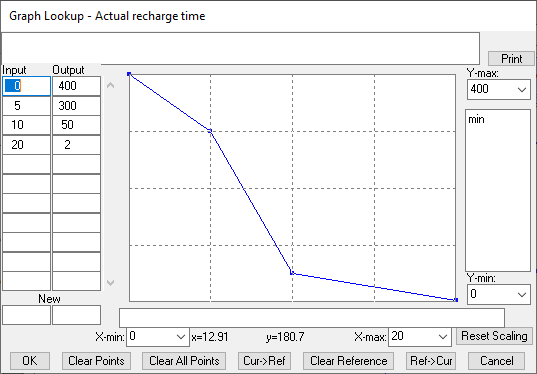
\includegraphics[width=0.89\linewidth]{img/recharge-time.png}
  \caption{Actual Recharge Time Data}
  \label{fig:recharge-time}
\end{subfigure}%
\begin{subfigure}{0.5\textwidth}
  \centering
  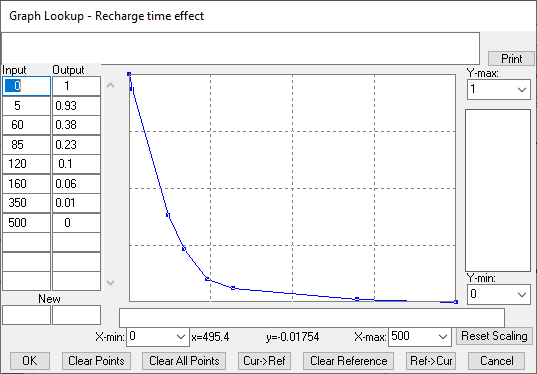
\includegraphics[width=0.89\linewidth]{img/recharge-time-effect.png}
  \caption{Recharge Time Effect Data}
  \label{fig:recharge-time-effect}
\end{subfigure}
\caption{Recharge Time Functions}
\label{fig:recharge-time-funcs}
\end{figure}

\subsubsection{Environmental Concern Effect}
More and more people are concerned with the future of our planet, so, this concern has an impact on EV sales. As can be seen in figure \ref{fig:env-concern}, at early stages this concern has a boost effect on sales around 5\%, this value starts to increase at fast pace in the next 12,5 years and then, as EVs become more and more common, its growth starts to slow down due to the loss of the novelty effect and the loss of the big disruption impact on people's lives and pollution percentages.

\begin{figure}[htbp]
\centerline{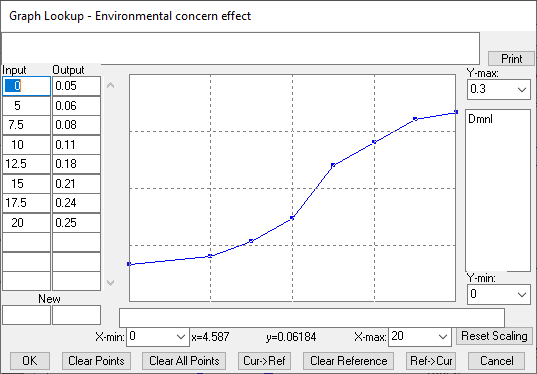
\includegraphics[width=0.45\linewidth]{img/env-concern-effect.png}}
\caption{Environmental Concern Effect}
\label{fig:env-concern}
\end{figure}

\subsection{Weight of Factors}
This section shows how each factor influence is weighed on the implemented model. Table \ref{table:factors-weights} summarizes how the weight is distributed among all the factors.

\begin{table}[htbp]
\centering
\begin{adjustbox}{width=0.8\textwidth}
\begin{tabular}{ccccccc}
\cline{2-6}
\multicolumn{1}{l|}{} & \multicolumn{1}{l|}{\textbf{Driving Range}} & \multicolumn{1}{l|}{\textbf{Charging Time}} & \multicolumn{1}{l|}{\textbf{Price Difference}} & \multicolumn{1}{l|}{\textbf{Recharge Infrastructure}} & \multicolumn{1}{l|}{\textbf{Environmental Concern}} \\ \cline{1-6}
\multicolumn{1}{|l|}{\textbf{Weight}} & \multicolumn{1}{c|}{0.3} & \multicolumn{1}{c|}{0.06} & \multicolumn{1}{c|}{0.56} & \multicolumn{1}{c|}{0.04} & \multicolumn{1}{c|}{0.04} \\ \cline{1-6}
\end{tabular}
\end{adjustbox}
\caption{Weight of Factors in Vensim Model}
\label{table:factors-weights}
\end{table}

\subsection{Summary of Model Variables}
Table \ref{fig:vensim-model} summarizes the entire model, listing all variables with its equations/initial values and units.

\begin{table}[!htpb]
   \centering
   \begin{adjustbox}{width=0.96\textwidth}
   \begin{tabular}{|l|l|l|}
   \hline
   \textbf{Variable} & \textbf{Equation/ Initial Value} & \textbf{Units} \\\hline
   INITIAL TIME & \textit{0} & \textit{Year} \\\hline
   FINAL TIME & \textit{20} & \textit{Year} \\\hline
   Potential Adopters & \makecell[l]{\textit{INTEG(Discard Rate - Rate of Adoption, \num{6.5e+6})}} & \textit{Person} \\\hline
   Rate of Adoption & \makecell[l]{\textit{Total adopters from Driving Range + Adopters from ads + Total Adopters from Price + } \\ \textit{Total adopters from Recharge Infrastructure + Total adopters from Recharge Time +} \\ \textit{ + Total adopters from Environmental Concern + Adopters from Word of Mouth}} & \textit{Person} \\\hline
   Adopters & \textit{INTEG(Rate of Adoption - Discard Rate, 16 000)} & \textit{Person} \\\hline
   Average EV lifetime & \textit{15} & \textit{Year} \\\hline
   Discard Rate & \textit{ 0.003 * ( Rate of Adoption / Average EV lifetime)} & \textit{Person} \\\hline
   Potential adopters per year & \textit{200 000} & \textit{Person/Year} \\\hline
   Environmental concern effect & \makecell[l]{\textit{WITH LOOKUP (Time,} \\
   \textit{([(0,0)-(20,0.3)],(0,0.05),(5,0.06),(7.5,0.08),(10,0.11),(12.5,0.18),(15,0.21),(17.5,0.24),(20,0.25) ))}} & \\\hline
   Adopters from environmental concern & \textit{Environmental concern effect * Potential adopters per year} & \textit{Person} \\\hline
   factor environmental concern & \textit{0.04} & \\\hline
   Total adopters from Environmental Concern &  \textit{factor environmental concern * Adopters from environmental concern} & \textit{Person} \\\hline
   Actual driving range & \makecell[l]{\textit{WITH LOOKUP (Time,} \\
   \textit{([(0,0)-(20,700)],(0,250),(5,300),(10,400),(16,550),(20,675) ))}} & Km \\\hline
   Driving range effect & \makecell[l]{\textit{WITH LOOKUP (Actual driving range,} \\ \textit{([(150,0)-(800,1)],(150,0.03),(200,0.05),(260,0.1),(440,0.42),(660,0.8),(800,0.95) ))}} & \\\hline
   Adopters from Driving Range & \textit{Driving range effect * Potential adopters per year} & \textit{Person} \\\hline
   factor driving range & \textit{0.3} & \\\hline
   Total adopters from Driving Range & \textit{factor driving range * Adopters from Driving Range} & \textit{Person} \\\hline
   Actual fixed costs difference & \makecell[l]{\textit{WITH LOOKUP (Time,} \\ \textit{([(0,0)-(20,10000)],(0,10000),(2.5,7500),(5,5750),(10,4500),(15,2900),(20,1900) ))}} & \textit{\euro} \\\hline
   Fixed costs difference effect & \makecell[l]{\textit{WITH LOOKUP (Actual fixed costs difference,} \\ \textit{([(-10000,0)-(10000,1)],(-10000,0.98),(-7000,0.95),(-6000,0.92),(-5400,0.89),(-3761} \\ \textit{,0.8246),(-2000,0.74),(-400,0.66),(-200,0.62),(0,0.33),(200,0.3),(400,0.29),(900,0.27} \\ \textit{),(1100,0.25),(1800,0.18),(2500,0.14),(3200,0.08),(4100,0.05),(5000,0.03),(10000,0) ))}} & \\\hline
   Actual variable costs difference & \makecell[l]{\textit{WITH LOOKUP (Time,} \\ \textit{([(0,-1000)-(20,1000)],(0,912),(13,0),(20,-707) ))}} & \textit{\euro} \\\hline
   Variable costs difference effect & \makecell[l]{\textit{WITH LOOKUP (Actual variable costs difference,} \\ \textit{([(-5000,0)-(5000,1)],(-5000,1),(-3000,0.93),(-800,0.63),(100,0.12),(400,0.07),(2100,0.01),(5000,0) ))}} & \\\hline
   Adopters from costs & \textit{(Fixed costs difference effect + Variable costs difference effect) * Potential adopters per year} & \textit{Person} \\\hline
   factor price difference & \textit{0.56} & \\\hline
   Total adopters from Price & \textit{factor price difference * Adopters from costs} & \textit{Person} \\\hline
   Advertising effect & \textit{0.00025} & \\\hline
   Adopters from ads & \textit{Advertising effect * Potential Adopters} & \textit{Person} \\\hline
   Actual recharge infrastructure density & \makecell[l]{\textit{WITH LOOKUP (Time,} \\ \textit{([(0,0)-(20,100)],(0,100),(2,60),(5,27),(10,10),(20,0) ))}} & \\\hline
   Recharge infrastructure density effect & \makecell[l]{\textit{WITH LOOKUP (Actual recharge infrastructure density,} \\ \textit{([(0,0)-(100,1)],(0,1),(2,0.99),(10,0.92),(18.35,0.8289),(26.61,0.6798),(33.94,0.5658),(42.2,0.5088)} \\ \textit{,(48.32,0.4561),(52.6,0.364),(57.19,0.2763),(64,0.24),(73.5,0.19),(91.3,0.125),(100,0) ))}} & \\\hline
   Adopters from recharge infrastructure & \textit{Recharge infrastructure density effect * Potential adopters per year} & \textit{Person} \\\hline
   factor recharge infrastructure & \textit{0.04} & \\\hline
   Total adopters from Recharge Infrastructure & \textit{factor recharge infrastructure * Adopters from recharge infrastructure} & \textit{Person} \\\hline
   Contact rate & \textit{Potential Adopters / Adopters} & \\\hline
   Adoption fraction & \textit{0.01} & \\\hline
   Total population & \textit{\num{1.028e+07}} & \textit{Person} \\\hline
   Adopters from Word of Mouth & \textit{Total population / Contact rate * Adoption fraction} & \textit{Person} \\\hline
   Actual driving range & \makecell[l]{\textit{WITH LOOKUP (Time,} \\
   \textit{([(0,0)-(20,400)],(0,400),(5,300),(10,50),(20,2) ))}} & min \\\hline
   Recharge time effect & \makecell[l]{\textit{WITH LOOKUP (Actual recharge time,} \\ \textit{([(0,0)-(500,1)],(0,1),(5,0.93),(60,0.38),(85,0.23),(120,0.1),(160,0.06),(350,0.01),(500,0) ))}} & \\\hline
   Adopters from Recharge time & \textit{Recharge time effect * Potential adopters per year} & \textit{Person} \\\hline
   factor recharge time & \textit{0.06} & \\\hline
   Total adopters from Recharge Time & \textit{factor recharge time * Adopters from Recharge time} & \textit{Person} \\\hline
   \end{tabular}
   \end{adjustbox}
   \caption{Model Summary | variables and functions}
   \label{table:model-summary}
\end{table}

\clearpage